\subsection{Random Walks}

A \emph{random walk}, a term first introduced in~\cite{pearson1905problem},
is a sequence of elements or a path on a mathematical space
produced by a random process. Among other applications, random walks are used
for sampling large graphs of social networks.
At a high level, a random walk in a graph is a sequence of nodes. This sequence
can be thought of as a sentence where each `node' is a `word'. Therefore, this
analogy lets us directly use techniques of word embeddings, for obtaining
embeddings of the nodes. In the next two sections, we introduce
two algorithms that use random walks to learn embeddings of the nodes
by applying an approach that was introduced for learning word embeddings.

\subsubsection{DeepWalk}

DeepWalk is an algorithm that takes a graph as an input, and learns a latent
representation of the nodes. This representation is a vector with continuous
values. The goal is for this representation to capture the social similarity
between the nodes and have a low dimension. In order to learn this
representation, DeepWalk uses random walks and assumes that these walks can
capture well the similarity between nodes. First it produces random walks by
selecting a node $v_i$ uniformly at random, from the set of nodes $V$, as the
root of the random walk $W_{v_i}$. Then, it samples one node from the set of the
neighbor nodes of $v_i$ uniformly at random. The last step is now repeated for
each new sampled node until the walk reaches a specific length. Having $\gamma$
such random walks, DeepWalk adapts the word2vec approach for obtaining word
embeddings, by treating the random walks as sentences, and the nodes as words.

The \emph{word2vec} method, introduced in \cite{mikolov2013efficient}, is a
method for embedding words of a corpus in a subspace $\mathbb{R}^d$ so that
each embeddings of a specific word can be used to predict the context around this
word, i.e. the words within a window $w$ in a sentence. Specifically, we
want to calculate the probability of every word of the vocabulary being
within a window from the current word (Skip-gram method).
In order to do that, skip-gram parses the words of a given corpus and creates
pairs of words $(w_i, w_j)$ that are within a window $w$, in order to specify
that $w_i$ and $w_j$ are within this window, which means that the two words
are in the same context. Therefore, this method assumes that words that are
`close' inside a sentence, correspond to the same context. These pairs
$(w_i, w_j)$ can be then used as a training set, to train a model to predict the
`nearby' words based on the training set with high probability, i.e. maximizing
the likelihood of the training set. The key idea is that the training of this
model proposes an embedding for each word in the $\mathbb{R}^d$.
Using this embedding we can represent each word as a vector with dimension $d$
which captures the context similarity instead of using an one-hot vector of
dimension equal to the size of the vocabulary. The parameter $d$ is set by the
user and it can be tuned using a validation set.
% Explain homofilous

DeepWalk adapts the idea of word embeddings to graphs by treating the nodes as
words and random walks as sentences. Similarly to the language model, the goal
is to capture node similarity which can be then used for classifying them.
There is no justification about why random walks can capture community
similarity information in a social network graph. However, the authors
%that random walks have been used for capturing
%similarities in a variety of problems. They also
observe that word frequency in some corpora, such as the English Wikipedia,
follows a power-law distribution, which is also the case for the degree of nodes
in social networks and that
possibly makes the random walk suitable for capturing the neighborhood
similarity and community membership in the social network graphs.

DeepWalk initializes a mapping
$\Phi: \mathbb{R}^{\mid V \mid \times S} \to \mathbb{R}^{\mid V\mid \times d}$
where $S$ in the size of the features space. Then, using random walks DeepWalk
solves the following optimization problem:
\begin{align}
    \min_{\Phi}
        \left (-\log{Pr({v_{i-w},
                \ldots, v_{i-1}, v_{i+1},
                \ldots , v_{i+w}} \mid \Phi(v_i))}
        \right )
\end{align}
where $v_i$ is the node currently examined in the random walk and
$v_{i-w}, \ldots, \ldots, v_{i-1}, v_{i+1},\ldots, v_{i+w}$ are the nodes
within a window $w$ from the node $v_i$ in this walk. The gradient of the above
quantity with respect to $\Phi$ is
computed in order to update the mapping $\Phi$. In the end, DeepWalk outputs
the matrix $\Phi$.

\subsubsection{Node2vec}

Similarly to DeepWalk, \emph{Node2vec} (\cite{grover2016node2vec}) is a method
for learning latent representations of the nodes by using random walks and the
skip-gram. However, this method uses a different way of sampling neighbor
nodes during a random walk, in order to handle graphs that have more structural
equivalent nodes different that the ones that include highly interconnected
nodes.

Node2vec introduces two baselines cases for sampling neighbor nodes: the
Breadth-first Sampling (BFS) and the Depth-first Sampling (DFS).
The Breadth-first strategy samples a neighborhood for a node $v_i$ by
considering as neighbors, the nodes that have an immediate edge to $v_i$.
In contrast, Depth-first strategy considers as neighbors the nodes that are
one more edge away from $v_i$ each time a neighborhood needed should include
more than one node. As an example, consider the node $u$ in
Fig~\ref{sampling_strategies} (obtained by the original
paper~\cite{grover2016node2vec}). Sampling a neighborhood of size 3 using the
BFS strategy can give us the nodes $s_1, s_2, s_3$, while using the DFS strategy
can give us the nodes $s_4, s_5, s_6$.
\begin{figure}
\begin{center}
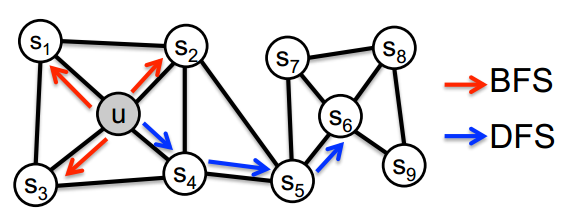
\includegraphics[width=0.7\textwidth]{figures/sampling.png}
\end{center}
\caption{Using the BFS sampling strategy, we can obtain the nodes
$s_1, s_2, s_3$ as the 3 neighbors of $u$. Using the DFS sampling strategy we
can obtain $\{s_4, s_5, s_6\}$. The figure is copied from the original
paper~\cite{grover2016node2vec}.}
\label{sampling_strategies}
\end{figure}
The BFS strategy can create random walks that capture the structural similarities
between nodes. For example, consider a network graphs with nodes that correspond
to hubs or bridges. In this case the embedding will reflect the structural
equivalence of the nodes of the graph.
On the contrary, the DFS strategy samples nodes in a way that explores
neighborhoods of nodes that exhibit \emph{homophily}, which means that nodes
highly connected belong to similar clusters/communities.

Real-world graph networks can be thought of as a mixture of networks that
include structural similar nodes and the ones networks that include nodes which
exhibit homophily. The node2vec approach tries to capture these similarities each
time based on the graph by introducing the parameters $p$, $q$. The return parameter $p$ controls the
likelihood of visiting the node already visited before the current node, or in
other words the likelihood of returning back to the node from which a node was
sampled as a neighbor. The parameter $q$ controls the decision between a BFS and
a DFS sampling strategy. If $q$ is less than 1 then the walk is more biased
to choose nodes that are further from the current node in the walk, while if $q$
is more than 1, then the walk would choose nodes that are close to the current
node with higher probability. Formally, the walk samples using the transition
probabilities $\pi_{ux}$ for going from a node $u$ to a node $x$:
\begin{align}
\pi_{ux} = \begin{cases} \frac{1}{p}\cdot w_{ux} & \text{ if } d_{tx} = 0 \\
1\cdot w_{ux} & \text{ if } d_{tx} = 1 \\
\frac{1}{q}\cdot w_{ux} & \text{ if } d_{tx} = 2
\end{cases}
\end{align}
where $t$ is the previous node in the random walk as shown in
Fig~\ref{node2vec_png} and $d_{tx}$ is the shortest path from $t$ to $x$.
\begin{figure}
\begin{center}
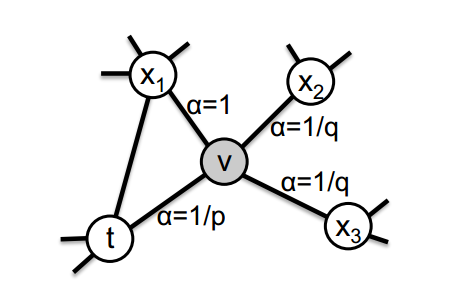
\includegraphics[width=0.5\textwidth]{figures/node2vec.png}
\end{center}
\caption{A random walk in the node2vec algorithm. The current node is the node
$v$ which was chosen as a neighbor to the vertex $t$.
Going back to $t$ is controlled by the parameter $p$, while going forward is
controlled by parameter $q$. The figure is copied from the original
paper~\cite{grover2016node2vec}.}
\label{node2vec_png}
\end{figure}

\subsubsection{LINE}

LINE (\cite{DBLP:journals/corr/TangQWZYM15}) is a network embedding model, able to handle very large, arbitrary types of graph networks $G=(V,E)$, (undirected, directed and/or weighted), by optimizing an objective which preserves both local and global network structures. Local structures are represented by the observed links in the networks, as for each pair of vertices linked by edge $(u, v)$, the weight $w_{uv}$ on that edge indicates the first-order proximity between u and v. Global structure is the second-order proximity between the vertices, determined through the shared neighborhood structures, as nodes with shared neighbors are likely to be similar. If $p_u = (w_{u,1}; \dots ;w_{u,|V|})$ denotes the first-order proximity of u with all the other vertices, then the second-order proximity between u and v is the similarity between $p_u$ and $p_v$.

In both cases, an objective function is defined and optimized, and the difference in the variants of the model that are described lies on whether first- or second-order proximity (or both) is used, and on the method selected for optimizing this objective in each case. Using first-order proximity, the KL-divergence between the joint and the empirical distribution of vertices $v_i$ and $v_j$ for each undirected edge $(i,j)$ is minimized. On the other hand, using second-order proximity, $u_i'$ is defined as the representation of $v_i$, when it is treated as a specific "context", and $u_i$ as the representation of $v_i$ when it is treated as a vertex. In this case, the KL-divergence between the conditional and the empirical distribution over the contexts is minimized.

A negative sampling approach tackles the problem of trivial infinity solutions in the case of first-order proximity and that of the computationally expensive minimization of the objective in the case of second-order proximity. Multiple negative edges are sampled according to some noisy distribution for each edge $(i,j)$, and asynchronous Stochastic Gradient Descent algorithm is used, which, in each step, samples a mini-batch of edges and updates the model parameters.
When edge weights have a high variance, scales of the gradients in SGD diverge, making it harder to find a good learning rate. Optimization via edge-sampling is then applied, by sampling from the original edges, with sampling probabilities proportional to the original edge weights. Sampled edges are treated as binary edges.

To combine first- and second-order proximity, a simple way is to concatenate the vector representations learned by both into a longer vector, and reweigh the dimensions, to balance the two representations. It was found that in practice, optimization takes $O(|E|)$ time, and the overall complexity of LINE is $O(d(K+1))$, given that K is the number of negative samples and $d<<|V|$ the dimension of the lower-dimensional space.

As a way to better combine first- and second-order proximities, the authors propose to jointly train the objective function in the future. Also, they suggest that higher-order proximity approaches could be applied to provide a better result. Another objective could be to find new embeddings of heterogeneous information networks, meaning graphs with vertices of multiple types. Furthermore, the case of no observed connections between new and existing vertices could be explored in the future by resorting to other network information, such as the textual information of the vertices.

\subsubsection{HARP}

HARP (\cite{DBLP:journals/corr/ChenPHS17}) is a meta strategy which solves the graph representation learning problem using a hierarchical approach.
All methods described before could easily get stuck at a bad local minima as the result of poor initialization of the non-convex optimization. Moreover,these methods mostly aim to preserve local proximities in a graph but neglect its global structure.

HARP recursively coalesces the nodes and edges in the original graph to get a series of successively smaller but structurally similar graphs . These coalesced graphs, each with a different granularity, provide a view of the original graph’s global structure. Starting from the most simplified form, each graph is used to learn a set of initial representations which serve as good initializations for embedding the next, more detailed graph. This process is repeated until we get an embedding for each node in the original graph.

HARP's method for multi-level graph representation learning consists of three parts:
\begin{itemize}
    \item \textbf{Graph Coarsening:} starting from the original graph, $G = G_0$, a hierarchy of successively smaller graphs $G_0, G_1, \dots , G_L$ is created. A hybrid graph coarsening scheme is developed, which is repeatedly applied to obtain a small graph. It combines two algorithms, edge collapsing and star collapsing, preserving first- and second-order proximity respectively. Edge collapsing is an edge selection and node merging algorithm, which arbitrarily merges nodes of edges into single nodes, providing a graph with at least half the edges of the original one. Star collapsing algorithm, on the other hand, considers star-like structured graphs, and merges nodes with the same neighbors into supernodes.
    \item \textbf{Graph Embedding:}  Using a provided Graph Embedding algorithm, Graph Embedding is obtained on the Coarsest Graph $G_L$, a small sized graph providing a high quality representation.
    \item \textbf{Representation Prolongation and Refinement:} For each graph $G_i$, the graph representation of $G_{i+1}$ is prolonged and taken as its initial embedding, $\Phi'_{G_i}$, followed by applying a provided embedding algorithm to $(G_i, \Phi'_{G_i})$ to further refine $\Phi'_{G_i}$ and obtain refined embedding $\Phi_{G_i}$.
\end{itemize}

Processes of Graph Embedding, Prolongation and Refinement are then applied recursively to the larger graphs and their embeddings, until we obtain the graph embedding of the original graph, $\Phi'_{G_0}$.

HARP is combined with a few state-of-the-art graph embedding methods (DeepWalk, LINE, Node2vec) to produce higher quality embeddings for all of them.
Time Complexity of HARP(DW) is the same as that of the original DeepWalk, equal to $O(\gamma |V|tw (d+dlog|V|))$, where $\gamma$ is the number of random walks, t is the  walk length, w is the window size, d is the representation size, and $|V|$ is the number of nodes. Similarly, time complexity of HARP(LINE) is the same as that of LINE, $O(r|E|)$,  linear to the number of edges in the graph, $|E|$, and the number of iterations over edges, r.
